\documentclass[11pt]{article}
%\usepackage{fullpage,url}
\usepackage{url}
\usepackage{amsmath}
\usepackage{graphicx}
\usepackage{caption}
\usepackage{subcaption}

\usepackage[letterpaper,top=1in,bottom=1in,left=1in,right=1in,nohead]{geometry}

\setlength{\parindent}{0in}
\setlength{\parskip}{6pt}
\bibliographystyle{plain}

\DeclareMathOperator{\E}{E}
\DeclareMathOperator{\Var}{Var}
\DeclareMathOperator{\Unif}{Unif}
\DeclareMathOperator{\shrink}{shrink}
\DeclareMathOperator{\Ncut}{Ncut}

\begin{document}
\thispagestyle{empty}
{\large{\bf CS7640: Advanced Image Processing \hfill Danny Perry}}\\

{\LARGE{\bf Segmentation using Normalized Cuts}}
\vspace{0.2\baselineskip}
\hrule

\section{Introduction}
Segmentation is one of the ongoing, fundamental problems in image processing and computer vision. 
There are essentially three ways to think about segmentation: classification of pixels, the delineation of boundaries, and partitioning the image into regions.
All three are useful mental models when thinking about the segmentation process, are all inter-related, and can be reformulated as each other.
Here I will be describing segmentation in the last form - that of partitioning the image into regions.

One interesting approach to segmentation is to model the image as a graph and make use of the extensive work in graph theory to solve the segmentation problem.
One approach using graph theory is to find a minimum graph cut to segment an image into regions - the goal being to choose a cut (and subsequent segmentation) so that the affinity of the different regions (segmentations) is minimized.

\cite{Shi2000} is a popular and interesting approach to using the minimum graph cut. 
Instead of using the standard graph cut, they normalize the cut using the association of each subgraph with the rest of the graph.
Normalizing the cut drives the solution to reject segmentations that only minimize the number of connections between the two subgraphs and focus more on the cut weights.
The method is straightforward and will be the primary subject of this report.

\section{Graph Construction}

In any of the methods making use of graph theory, a graph needs to be generated from the image information.
\cite{Shi2000} suggest a few specific methods to construct the connections and their weights.
In general their approach models the weights between two pixels like so:

\begin{equation*}
  w_{ij} = \exp(-||F(i)-F(j)||^2_2 / \sigma_I ) * 
  \begin{cases}
    \exp(-||X(i)-X(j)||^2_2 / \sigma_X ) \text{    if} ||X(i)-X(j)||_2 < r \\
    0 \text{  otherwise}
  \end{cases}
\end{equation*}

Where $F(\cdot)$ is some feature (such as the intensity of the pixel, or something derived from the intensity), $X(\cdot)$ is the location of the pixel, $r$ is the radius of connectivity of the pixel, and $\sigma_{\cdot}$ controls the width of the kernel.
As you can see, with a larger $r$, there is potential for more connectivity, and with a larger $\sigma$ there is potential for higher weights on any connecting edges.

\cite{Shi2000} specifically suggest some choices for $F(\cdot)$, for example, using $F(i)=I(i)$ for a grayscale image and $F(i) = [v,v \cdot s \cdot \sin(h), v \cdot s \cdot \cos(h)](i)$ for a color image (where $h,s,v$ are the HSV values.

Each of these choices has varying effect on the results.
For example Figure \ref{fig:radius} shows some different results using different values of $r$.
As mentioned above, a larger $r$ value provides more opporunity for connectivity - in other words, a larger neighborhood of pixels are considered as potential nodes to connect to.
The $r$ and $\sigma$ values are closely related and while $r$ controls the potential connections, $\sigma$ helps determine the weight on any connections.
For all of the examples here, I've chosen $\sigma = r/3$ to follow the semi-standard of having $r = 3*\sigma$ (support of a Gaussian).

As Figure \ref{fig:radius} shows, the larger radius in this case gives a much better segmentation.
Each of these cases use the second eigenvector for the segmentation.
Figure \ref{rad:r1} shows a very bad segmentation.
The pixels are not interconnected enough to establish any strong affinity.
There is still some general pattern to the segemntation (you can make out a background and a blob that is the bird and branches), but it is not a good segmentation.
Figure \ref{rad:r5} shows improvment by increasing the radius to $5$, while Figure \ref{rad:r10} shows the best segmentation with $r=10$.

The choice of $F(\cdot)$, also has some effect on the segmentation outcome.
Here we've mainly used $F(i)=I(i)$, but for color images we use the feature described above.
A result using a colored image is shown in Figure \ref{fig:res:ws} with decent results.
It would be interesting to compare the segmentations performed on the grayscale version of an image and compare to this color image feature.

As \cite{Shi2000} mentions, sometimes the eigenvectors need to be further filtered to ignore those that have a more continuous range of values.
This is because in order to make a good determination of which segment the pixel belongs to we want a clear separation of eigenvector values.
The lack of clear boundaries in Figure \ref{rad:r5} is both a product of the lack of connectivity and this smooth gradation of eigenvector values.
Figure \ref{fig:ev:r5} shows six different segmentations using $r=5$, as you can see some eigenvector choise come out clearer than others.
This is why the paper suggests restricting eigenvector choices to those with a "continuous" range of values.

\begin{figure}
\centering
\graphicspath{{../code/}}
\begin{subfigure}[b]{0.4\textwidth}
\centering
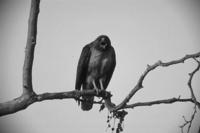
\includegraphics[width=\textwidth]{hawk_sm}
\caption{Original}
\label{rad:orig}
\end{subfigure}
\begin{subfigure}[b]{0.4\textwidth}
\centering
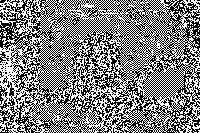
\includegraphics[width=\textwidth]{hawk_1_seg}
\caption{Segmentation with $r=1$}
\label{rad:r1}
\end{subfigure}
\begin{subfigure}[b]{0.4\textwidth}
\centering
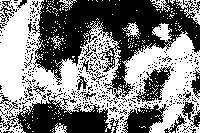
\includegraphics[width=\textwidth]{hawk_5_seg}
\caption{Segmentation with $r=5$}
\label{rad:r5}
\end{subfigure}
\begin{subfigure}[b]{0.4\textwidth}
\centering

\includegraphics[width=\textwidth]{hawk_10_seg}
\caption{Segmentation with $r=10$}
\label{rad:r10}
\end{subfigure}
\caption{Results of varying connectivity radius size $r$.}
\label{fig:radius}
\end{figure}


Figure \ref{fig:ev:r5} shows the segmentations based on the first 6 eigenvectors for the case where $r=5$.
(Note I will use the term "smallest eigenvector" to refer to the eigenvector associated with the smallest eigenvalue.)
You'll notice that Figure \ref{fig:ev4:r5} has the best segmentation outlier of any of them, but it still has some small noise effect, which the larger radius size seems to take care of.


\begin{figure}
\centering
\graphicspath{{../code/}}
\begin{subfigure}[b]{0.4\textwidth}
\centering
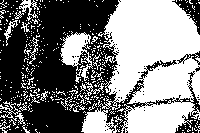
\includegraphics[width=\textwidth]{hawk_5_seg_ev1}
\caption{First eigenvector}
\label{fig:ev1:r5}
\end{subfigure}
\begin{subfigure}[b]{0.4\textwidth}
\centering
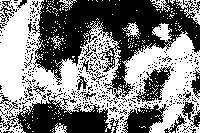
\includegraphics[width=\textwidth]{hawk_5_seg}
\caption{Second eigenvector}
\label{fig:ev2:r5}
\end{subfigure}
\begin{subfigure}[b]{0.4\textwidth}
\centering
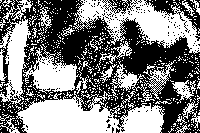
\includegraphics[width=\textwidth]{hawk_5_seg_ev3}
\caption{Third eigenvector}
\label{fig:ev3:r5}
\end{subfigure}
\begin{subfigure}[b]{0.4\textwidth}
\centering
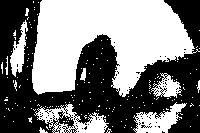
\includegraphics[width=\textwidth]{hawk_5_seg_ev4}
\caption{Fourth eigenvector}
\label{fig:ev4:r5}
\end{subfigure}
\begin{subfigure}[b]{0.4\textwidth}
\centering
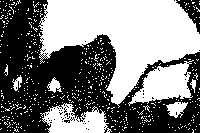
\includegraphics[width=\textwidth]{hawk_5_seg_ev5}
\caption{Fifth eigenvector}
\label{fig:ev5:r5}
\end{subfigure}
\begin{subfigure}[b]{0.4\textwidth}
\centering
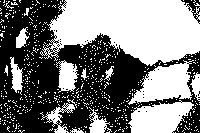
\includegraphics[width=\textwidth]{hawk_5_seg_ev6}
\caption{Sixth eigenvector}
\label{fig:ev6:r5}
\end{subfigure}
\caption{Results using different eigenvectors from the same Rayleigh coefficient with $r=5$.}
\label{fig:ev:r5}
\end{figure}


\section{Solution using Eigenanalysis}

Once the graph structure has been computed the edge weight matrix $W$ is used to compute the digonal matrix $D$ where each $d_{ii} = \sum_j w_{ij}$.

Using these two matrices, an approximation to the minimum normalized cut can be described in this way:

\begin{equation*}
  \min_x \Ncut(x) = \min_y \frac{y^T(D-W)y}{y^TDy}
\end{equation*}

Which is known as the Rayleigh quotient.
The approximation can then be computed by solving the generalized eigenvalue system

\begin{equation*}
  (D-W)y=\lambda Dy
\end{equation*}

And using the eigenvector associated with the second smallest eigenvalue as the partitioning vector.
Figures \ref{fig:ev:r5} and \ref{fig:ev:r10} show the result of using various other eigenvectors as the partitioning vector.
The paper suggests filtering the eigenvectors and not even consider those with a smooth range of values - because they correspond to segmentation that are ill-determined.

The eigenvectors are then converted into a segmentation using some kind of thresholding on the eigenvector.
The median value or $0$ are recommended in the paper, here I've used the median value as the threshold.

\begin{figure}
\centering
\graphicspath{{../code/}}
\begin{subfigure}[b]{0.4\textwidth}
\centering
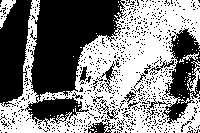
\includegraphics[width=\textwidth]{hawk_10_seg_ev1}
\caption{First eigenvector}
\label{fig:ev1:r10}
\end{subfigure}
\begin{subfigure}[b]{0.4\textwidth}
\centering

\includegraphics[width=\textwidth]{hawk_10_seg}
\caption{Second eigenvector}
\label{fig:ev2:r10}
\end{subfigure}
\begin{subfigure}[b]{0.4\textwidth}
\centering
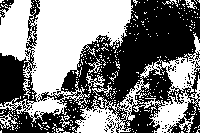
\includegraphics[width=\textwidth]{hawk_10_seg_ev3}
\caption{Third eigenvector}
\label{fig:ev3:r10}
\end{subfigure}
\begin{subfigure}[b]{0.4\textwidth}
\centering
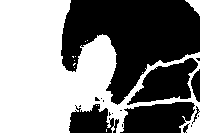
\includegraphics[width=\textwidth]{hawk_10_seg_ev4}
\caption{Fourth eigenvector}
\label{fig:ev4:r10}
\end{subfigure}
\begin{subfigure}[b]{0.4\textwidth}
\centering
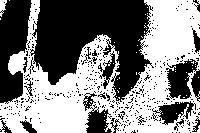
\includegraphics[width=\textwidth]{hawk_10_seg_ev5}
\caption{Fifth eigenvector}
\label{fig:ev5:r10}
\end{subfigure}
\begin{subfigure}[b]{0.4\textwidth}
\centering
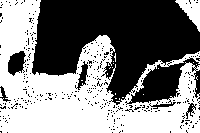
\includegraphics[width=\textwidth]{hawk_10_seg_ev6}
\caption{Sixth eigenvector}
\label{fig:ev6:r10}
\end{subfigure}
\caption{Results using different eigenvectors from the same Rayleigh coefficient with $r=10$.}
\label{fig:ev:r10}
\end{figure}

\section{Results}

The algorithm was run on a collection of images from \cite{berkeleyImages}.
Some results are shown in Figure \ref{fig:results}.

By far the most costly portion of the method is the graph construction.
This is because the the edge weight matrix is $N^2$ where $N=n^2$ is the number of pixels in an $n$ by $n$ image, which results in an $n^4$ size matrix for an $n$ by $n$ image.
Needless to say it becomes very large with any reasonably sized image.
With matrices that size, it's imperative to use a sparse matrix impelementation with corresponding linear algebra routines, like those available in Matlab.
Othewise the edge weight matrix becomes much larger than most contemporary main memory sizes.

With such an library the actual solution to the eigenvlue problem becomes fairly straight forward.

Overall this method is very straight forward and easy to understand, and reasonably easy to implement.
It's also very nice because of the lack of parameter tuning.  There's really only a single paramter - the size of the connectivity radius $r$.
There's also a little bit of filtering with the eigenvectors, but that can be done mostly automatically using histogram bin ratios, as described in the paper.
The only gotcha is figuring out an efficient way to construct the graph over the image in the first place.

 
\begin{figure}
\centering
\graphicspath{{../code/}}
\begin{subfigure}[b]{0.4\textwidth}
\centering
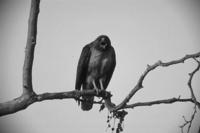
\includegraphics[width=\textwidth]{hawk_sm}
\caption{Hawk Original}
\label{fig:ev1:r10}
\end{subfigure}
\begin{subfigure}[b]{0.4\textwidth}
\centering

\includegraphics[width=\textwidth]{hawk_10_seg}
\caption{Hawk Segmentation}
\label{fig:ev2:r10}
\end{subfigure}
\begin{subfigure}[b]{0.4\textwidth}
\centering
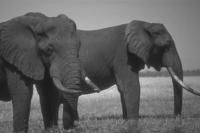
\includegraphics[width=\textwidth]{elephants_sm}
\caption{Elephant Original}
\label{fig:ev3:r10}
\end{subfigure}
\begin{subfigure}[b]{0.4\textwidth}
\centering
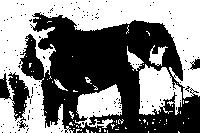
\includegraphics[width=\textwidth]{elephants_seg_ev4}
\caption{Elephant Segmentation}
\label{fig:ev4:r10}
\end{subfigure}
\begin{subfigure}[b]{0.4\textwidth}
\centering
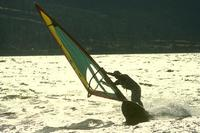
\includegraphics[width=\textwidth]{windsurf_sm}
\caption{Windsurfer Original}
\label{fig:ev5:r10}
\end{subfigure}
\begin{subfigure}[b]{0.4\textwidth}
\centering
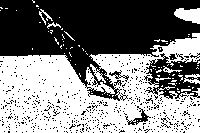
\includegraphics[width=\textwidth]{windsurf_seg_ev6}
\caption{Windsurfer Segmentation}
\label{fig:res:ws}
\end{subfigure}
\caption{Results on some sample images.}
\label{fig:results}
\end{figure}

\section{Conclusions}

Here I've presented the normalized graph cut method for segmentation.
I've shown the effect of the primary parameter $r$, as well as some of the subtelty associated with filtering the eigenvectors.
Another area of parameter or model decision that wasn't investigated here is in the determination of the features used to decide affinity between two pixels.
The paper briefly mentions this choice, but doesn't go into any detail.
It would be interesting to investigate the effects of that choice, specifically for difficult images to segment.
Since normalized cuts method is sensitive to this affinity calculation (as shown by the different choices of $r$), it would make sense that a careful choice of $F(\cdot)$ could dramatically improve the results on a difficult data set.
Here I've shown reasonable results on real images from a public segmentation data set.
Overall I found that this method is both straightforward and fairly easy to implement, while doing an effective segmenting job.

\bibliography{normalized_cuts}

\end{document}
